%!TEX root = ../dokumentation.tex

%TODO: Einleitung überarbeiten
\chapter{Implementierung}\label{cha:Implementierung}
\section{Datenbank, Login und Registrierung}\label{Datenbank}
Zu Beginn verbindet sich der Server mit der Datenbank. Server und Datenbank können über einen definierten Port kommunizieren. Der Server kann mittels Datenbankabfragen auf die Daten zugreifen. Wenn sich ein neuer User registriert, sendet der Client dem Server den Usernamen und das Passwort. Der Server fordert nun von der Datenbank gespeicherte Daten an, die den Usernamen und das Passwort enthalten. Wenn die Antwort der Datenbank ein leeres Objekt ist, ist noch kein User mit dem Usernamen und dem Passwort registriert und in der Datenbank wird ein neuer Eintrag erstellt. 

Folgendes Bild zeigt den Ablauf des Logins:
\begin{figure}[H]
\centering
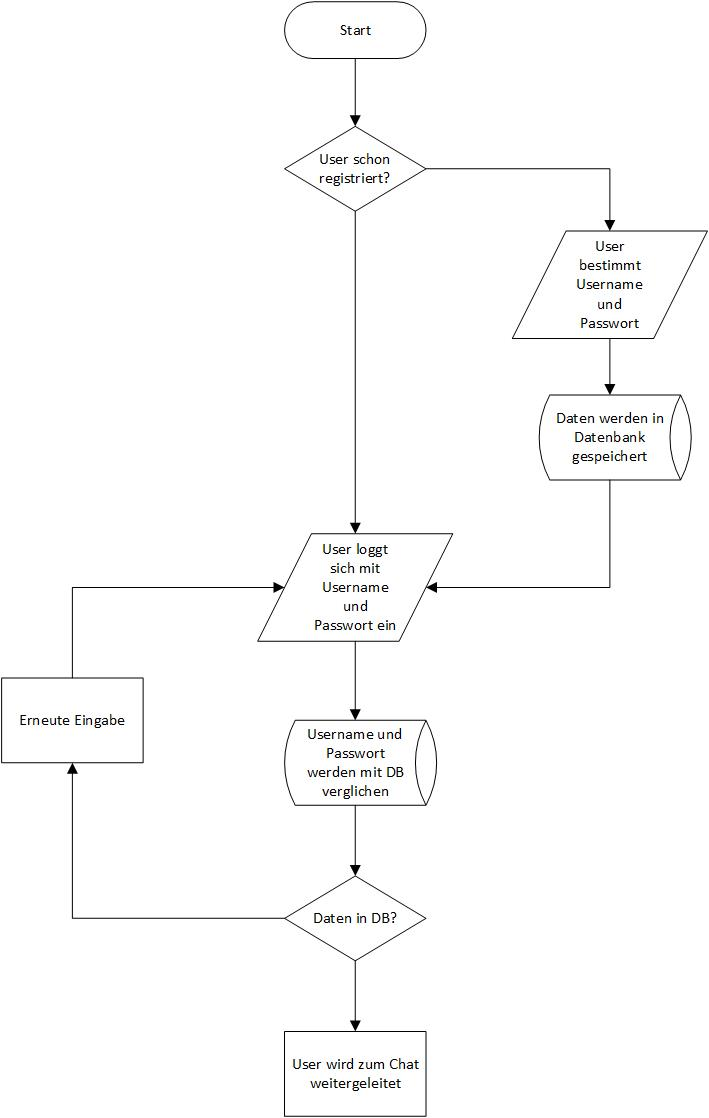
\includegraphics[width=0.5\textwidth]{images/login.jpg}
\caption{Flussdiagramm des Loginprozesses}
\end{figure}


\section{Spiellogik}\label{sec:Spiellogik}
\section{Erkennung des Spielendes}\label{sec:GameOver}
Es gibt zwei Szenarien, unter denen das Spiel zu Ende ist. Entweder gewinnt ein Spieler oder das Spiel endet unentschieden. Unentschieden ist das Spiel, wenn das Spielfeld komplett gefüllt ist, aber kein Spieler eine Reihe aus vier Steinen aufbauen konnte.
Bei einem Gewinn sind drei verschiedene Szenarien zu unterscheiden. Eine Reihe aus vier Spielsteinen des gleichen Spielers kann horizontal, vertikal oder diagonal auftreten. Wenn die Reihe diagonal gebildet wird, kann noch zwischen von links unten nach rechts oben und von rechts unten nach links oben unterschieden werden. Alle diese Fälle müssen geprüft werden.

\section{Docker Compose}\label{sec:Docker Compose}
Im Docker-Compose-File sind die zu verwaltenen Container aufgezählt mitsamt der Portnummern, über den auf die Container zugegriffen werden kann.


